\section{Configuration file}
\label{S:CFGFile}
The configuration file is a \MATLAB{} script utilized for initializing the project (see Figure \ref{fig:cfgfile}).
The name of a configuration file can be given as an input to the function   \lstinline[basicstyle = \mlttfamily \small ]!OpenBLDM_main.m!, as mentionned in Section~\ref{SS:OpenBDLMinput}.
The configuration file must follow a specific structures, which includes 6 sections: Project name, Data, Model structure, Model parameters, Initial states values and Options.
The first three sections are mandatory, while the last three sections are optional.
\begin{figure}[h!]
\centering
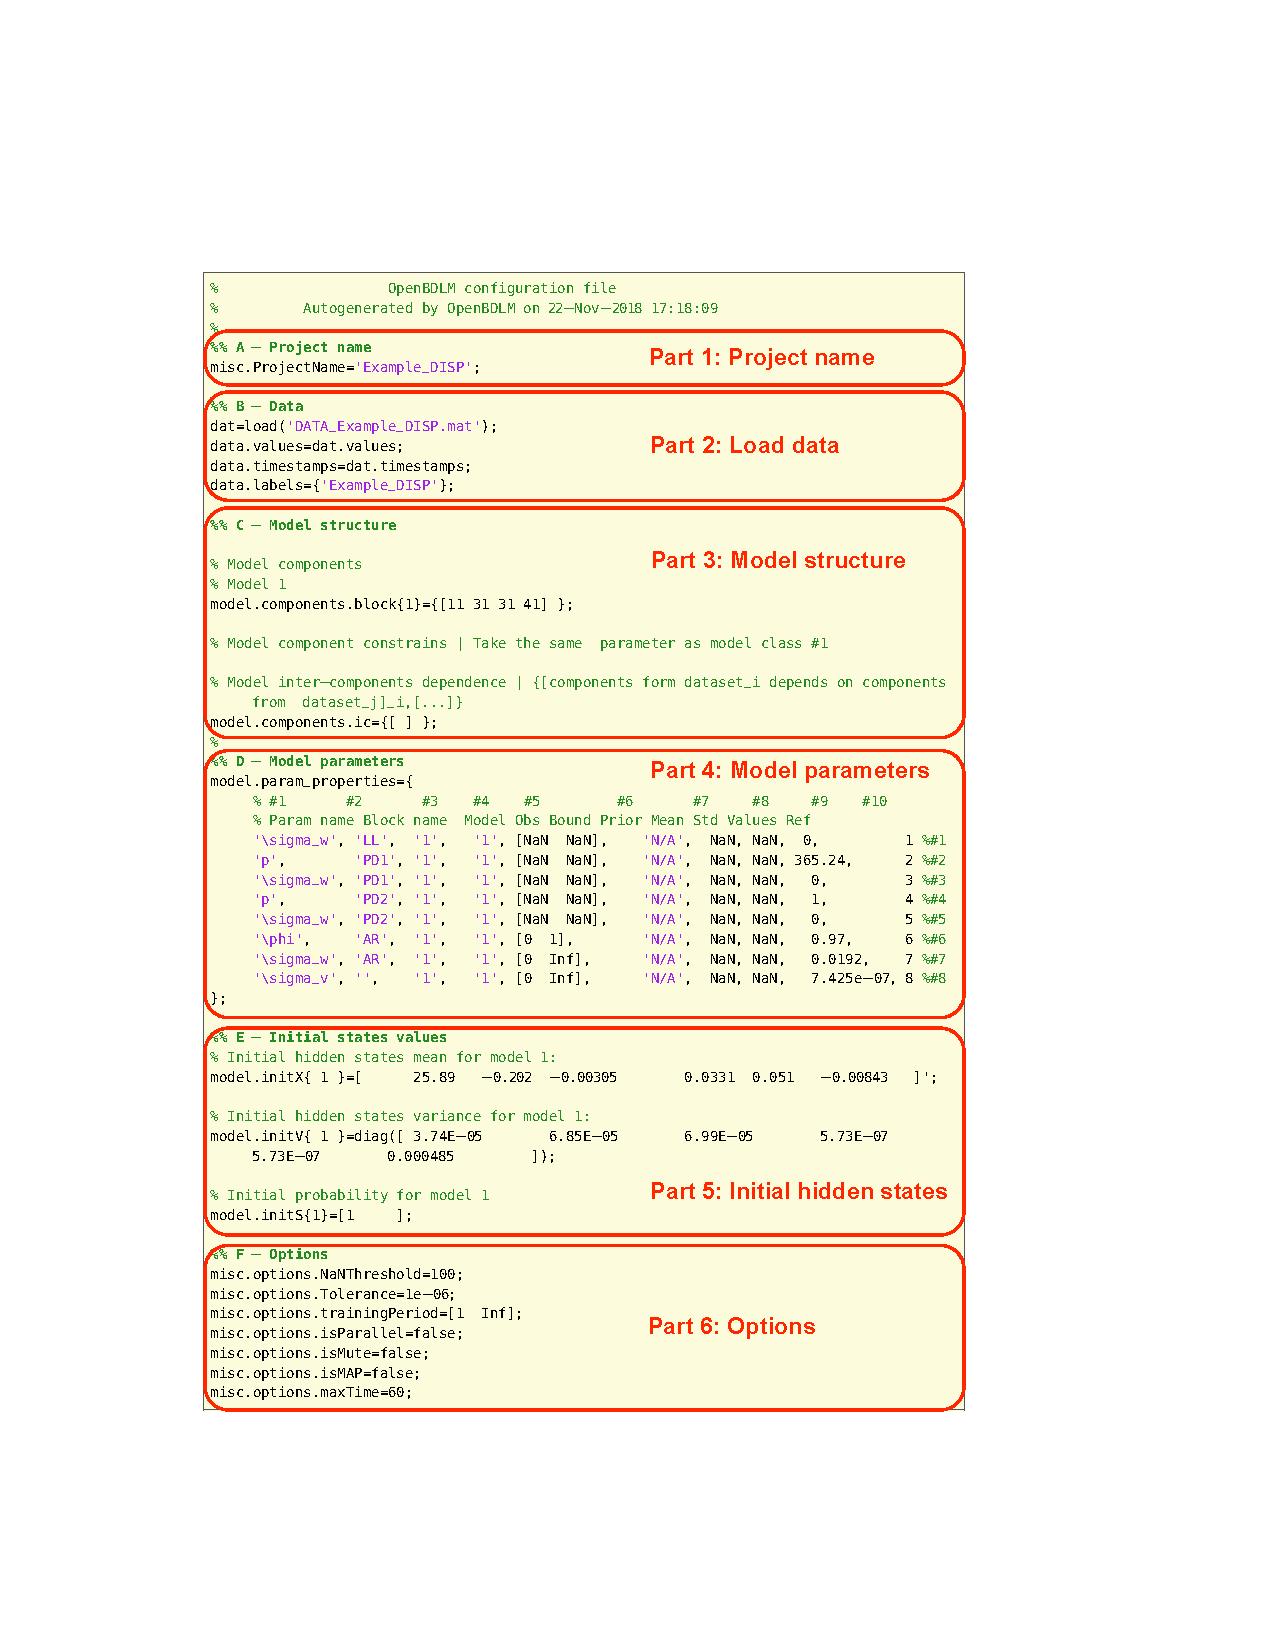
\includegraphics[width=140mm]{docfigs/Example_DISPSIM/listing/config_file_1.pdf}
\caption{Exemple of configuration file}
\label{fig:cfgfile}
\end{figure}

\subsection{Project name}
This section of the configuration file defines the name of the project as a vector of characters stored in the field \lstinline[basicstyle = \mlttfamily \small ]!ProjectName! of the \MATLAB{} variable \lstinline[basicstyle = \mlttfamily \small ]!misc!.

\subsection{Data}

This section of the configuration file defines information required for loading the data from a \lstinline[basicstyle = \mlttfamily \small ]!DATA_! file located in ``/data/mat'' subfolder.
The file must follow the format described in Section~\ref{SS:MATInput}.
The timestamp values, the amplitude values and the label values must be stored in the fields \lstinline[basicstyle = \mlttfamily \small]!timestamps!, \lstinline[basicstyle = \mlttfamily \small]!values!, and \lstinline[basicstyle = \mlttfamily \small]!labels! of the \MATLAB{} structure named \lstinline[basicstyle = \mlttfamily \small]!data!.

\subsection{Model structure}
\label{SS:ModelComponents}
This part of the configuration file defines the model in a \MATLAB{} structure named \lstinline[basicstyle = \mlttfamily \small]!model.component!.
The structure \lstinline[basicstyle = \mlttfamily \small]!model.component! must have three fields, named \lstinline[basicstyle = \mlttfamily \small]!model.component.block!, \lstinline[basicstyle = \mlttfamily \small]!model.component.ic!, and \lstinline[basicstyle = \mlttfamily \small]!model.component.const!.

\begin{itemize}

\item \lstinline[basicstyle = \mlttfamily \small ]!model.component.block!: it defines the block components associated with each time series.
The field \lstinline[basicstyle = \mlttfamily \small ]!block! stores $1\times \mathtt{S}$ cell array, where $\mathtt{S} = \{1,2 \}$ is the number of model classes.
Each cell array is a $1\times \mathtt{D}$ cell array of matrice, where $\mathtt{D}$ is the number of time series.
Each block component is associated with a reference number:
\begin{itemize}
\item 11: Local level 
\item 12: Local trend
\item 13: Local acceleration
\item 21: Local level compatible with local trend
\item 22: Local level compatible with local acceleration
\item 23: Local trend compatible with local acceleration
\item 31: Periodic
\item 41: First-order autoregressive
\item 51: Kernel regression
\item 61: Level intervention
\end{itemize}

\item  \lstinline[basicstyle = \mlttfamily \small ]!model.component.const!: it constrains model parameters between the block components from different model classes.
The field \lstinline[basicstyle = \mlttfamily \small ]!const! stores a $1\times \mathtt{S}$ cell array, where $\mathtt{S} = \{1, 2 \}$ is the total number of model classes.
It is defined only if $\mathtt{S} = 2$.
The first cell is empty, and the second cell is a $1\times \mathtt{D}$ cell array of array, where $\mathtt{D}$ is the number of time series.
The array contains $0$ and $1$ to indicate which block components of the second model class has the same model parameters than the corresponding component of the first model class. 
A value of $1$ indicates that the model parameters are constrained between the block components of the two model classes, $0$ otherwise.

\item  \lstinline[basicstyle = \mlttfamily \small ]!model.component.ic!:  it defines the dependencies among the time series.
The field \lstinline[basicstyle = \mlttfamily \small ]!ic! stores a $1\times \mathtt{D}$ cell array of $1\times (\mathtt{D}-1)$ matrix, where $\mathtt{D}$ is the number of time series.
Each time series depend on the time series corresponding to the indexes given in the $\mathtt{D}$ arrays.
If the array is empty, the time series are considered independent by default.

\end{itemize}


\subsection{Model parameters}
\label{SS:ModelParamProperties}
This part of the configuration file aims at defining the model parameter properties which are stored in the field named \lstinline[basicstyle = \mlttfamily \small ]!model.param_properties! of the \MATLAB{} structure \lstinline[basicstyle = \mlttfamily \small ]!model!.
The field \lstinline[basicstyle = \mlttfamily \small ]!model.param_properties! stores $\mathtt{K} \times 10$ cell array, where $\mathtt{K}$ is the total number of model parameters.
\begin{itemize}
\item column 1 must be a character vector that gives the name of the model parameters (e.g.  \lstinline[basicstyle = \mlttfamily \small ]!sigma_w!). 
\item column 2 must be a character vector that gives the reference name of the block associated with the parameter (e.g \lstinline[basicstyle = \mlttfamily \small ]!LL!, see Section~\ref{SS:BlockComponent}).
\item column 3 must be a character vector that gives the index corresponding to the model class associated with the parameter (e.g  either \lstinline[basicstyle = \mlttfamily \small ]!1! or \lstinline[basicstyle = \mlttfamily \small ]!2!) (see~\ref{SS:THSKF}).
\item column 4 must be a character vector that gives the index corresponding to the observation associated with the parameter (e.g \lstinline[basicstyle = \mlttfamily \small ]!3!).
\item column 5 must be a $1\times2$ array that gives the bound of the parameter (e.g \lstinline[basicstyle = \mlttfamily \small ]![NaN, NaN]!,  \lstinline[basicstyle = \mlttfamily \small ]![0, Inf]!, \lstinline[basicstyle = \mlttfamily \small ]![0, 1]!). 
The bounds are used to transform (if necessary) model parameters from a bounded to  an unbounded space during the optimization process (see Sections~\ref{S:PARAMESTIMATION} and~\ref{SS:THModelParameterEstimation}).
\item column 6 must be a character vector that gives the type of the prior used during the optimization process (e.g  either \lstinline[basicstyle = \mlttfamily \small ]!N/A! or \lstinline[basicstyle = \mlttfamily \small ]!normal!). 
\lstinline[basicstyle = \mlttfamily \small ]!N/A! indicates that no prior is used (see Sections~\ref{S:PARAMESTIMATION} and~\ref{SS:THModelParameterEstimation}).
\item column 7 must be a real number that gives the mean of the prior when a prior of type \lstinline[basicstyle = \mlttfamily \small ]!normal! is used, otherwise it must be set to \lstinline[basicstyle = \mlttfamily \small ]!NaN! (see Sections~\ref{S:PARAMESTIMATION} and~\ref{SS:THModelParameterEstimation}).
\item column 8 must be a real number that gives the standard deviation of the prior when a prior of type \lstinline[basicstyle = \mlttfamily \small ]!normal! is used, otherwise it must be set to \lstinline[basicstyle = \mlttfamily \small ]!NaN! (see Sections~\ref{S:PARAMESTIMATION} and~\ref{SS:THModelParameterEstimation}).
\item column 9 must be a real number that gives the value of the model parameters.
\item column 10 must be an integer that gives the reference number of the model parameters. The model parameters which share the same reference number are constrained to each other.
\end{itemize}

\subsection{Initial states values}
\label{SS:InitialHS}
This part of the configuration file defines the initial states values (at time $t=0$).
The initial mean and covariance hidden states values are stored in the \lstinline[basicstyle = \mlttfamily \small ]!model.initX! and \lstinline[basicstyle = \mlttfamily \small ]!model.initV! fields.
The initial probability for the model class is stored in the field \lstinline[basicstyle = \mlttfamily \small ]!model.initS!.

\begin{itemize}
\item \lstinline[basicstyle = \mlttfamily \small ]!model.initX!: $1\times \mathtt{S}$ cell array of array, where $\mathtt{S} \in \{1, 2 \}$ is the total number of model classes.
Each array is $\mathtt{L}\times1$ array of real number that stores the initial mean values associated with each hidden states variables, where $\mathtt{L}$ is the total number of hidden states variables associated with the model.
\item \lstinline[basicstyle = \mlttfamily \small ]!model.initV!: $1\times \mathtt{S}$ cell array of array, where $\mathtt{S} \in \{1, 2 \}$ is the total number of model classes.
Each array is $\mathtt{L}\times\mathtt{L}$ array of real number that stores the initial variance and covariances values associated with each hidden states variables.
\item \lstinline[basicstyle = \mlttfamily \small ]!model.initS!: $1\times \mathtt{S}$ cell array of array, where $\mathtt{S} \in \{1, 2 \}$ is the total number of model classes. 
Each array is $1\times1$ array of real number that gives the initial probability for the model class.
\end{itemize}

\subsection{Options}
\label{SS:options}
This part of the configuration file defines the options that control different aspect of the software regarding the data pre-processing, optimization, hidden states estimation, and aspects related to graphical outputs.
The options are stored in the field named \text{options} of the \MATLAB{} variable \lstinline[basicstyle = \mlttfamily \small ]!misc!.
\begin{itemize}

\item Options for the data pre-processing

\begin{itemize}
\item \lstinline[basicstyle = \mlttfamily \small ]!misc.options.NaNThreshold!: real number that gives, in percent, the amount of missing data allowed at each time slice.\\Default: \lstinline[basicstyle = \mlttfamily \small ]!100!.
\item \lstinline[basicstyle = \mlttfamily \small ]!misc.options.Tolerance!: real number that gives the duration (in number of days) after which two timestamps are not considered equal. \\Default: $10^{-6}$.

\end{itemize}


\item Options for the model parameters estimation

\begin{itemize}
\item \lstinline[basicstyle = \mlttfamily \small ]!misc.options.trainingPeriod!:  $1\times2$ array of real number that defines the training period, given in number of days since the first timestamp. \\Default: \lstinline[basicstyle = \mlttfamily \small ]![1 Inf]!. 
\item \lstinline[basicstyle = \mlttfamily \small ]!misc.options.isParallel!: logical that triggers or not the parallel computation for approximating the gradient in the optimization procedure. Note that parallel computation requires the \MATLAB{} \emph{Parallel Computing Toolbox}. \\Default: \lstinline[basicstyle = \mlttfamily \small ]!true!.
\item \lstinline[basicstyle = \mlttfamily \small ]!misc.options.maxIterations!: integer that gives the maximum number of iterations for the optimization procedure. Newton-Raphson only. \\Default: \lstinline[basicstyle = \mlttfamily \small ]!100!.
\item \lstinline[basicstyle = \mlttfamily \small ]!misc.options.maxTime!: real number that gives, in minutes, the maximum amount of  time to spend for the optimization procedure. \\Default: \lstinline[basicstyle = \mlttfamily \small ]!60!.
\item \lstinline[basicstyle = \mlttfamily \small ]!misc.options.isMAP!: logical that triggers or not the Maximum A Posteriori (MAP) estimation of the model parameters during the optimization procedure. MAP estimation includes prior information about the model parameters. \\Default: \lstinline[basicstyle = \mlttfamily \small ]!false!.
\item \lstinline[basicstyle = \mlttfamily \small ]!misc.options.isPredCap!: logical so that if \lstinline[basicstyle = \mlttfamily \small ]!isPredCap=true!, the Prediction Capacity (i.e. the log-likelihood over a test dataset) is used to drive the optimization process, otherwise the log-likelihood over the full dataset is used. This option is used only for Stochastic Gradient optimization. \\Default: \lstinline[basicstyle = \mlttfamily \small ]!false!.
\item \lstinline[basicstyle = \mlttfamily \small ]!misc.options.isLaplaceApprox!: logical so that if \lstinline[basicstyle = \mlttfamily \small ]!isLaplaceApprox=true! the posterior covariance matrix is estimated using Laplace approximation around the optimized model parameters values. This option is used only for Newton-Raphson optimization. \\Default: \lstinline[basicstyle = \mlttfamily \small ]!false!.
\item \lstinline[basicstyle = \mlttfamily \small ]!misc.options.NRTerminationTolerance!: real value determining the termination tolerance for the Newton-Raphson algorithm. \\Default: $10^{-7}$.
\item \lstinline[basicstyle = \mlttfamily \small ]!misc.options.NRLevelsLambdaRef!: integer that controls the number of trial loop for a parameter being optimized for theNewton-Raphson algorithm. \\Default: $4$.
\item \lstinline[basicstyle = \mlttfamily \small ]!misc.options.isMute!: logical so that if \lstinline[basicstyle = \mlttfamily \small ]!isMute=true!, no message are displayed on screen during the optimization procedure. \\Default: \lstinline[basicstyle = \mlttfamily \small ]!false!.
\item \lstinline[basicstyle = \mlttfamily \small ]!misc.options.maxEpochs!: integer that gives the maximum number of epochs the optimization procedure. This option is used only for Stochastic Gradient optimization. \\Default: \lstinline[basicstyle = \mlttfamily \small ]!50!.
\item \lstinline[basicstyle = \mlttfamily \small ]!misc.options.Optimizer!: vector of character that defines the optimizer for Stochastic Gradient algorithm. It must be either \lstinline[basicstyle = \mlttfamily \small ]!'MMT'!, \lstinline[basicstyle = \mlttfamily \small ]!'ADAM'!, \lstinline[basicstyle = \mlttfamily \small ]!'MMTbeta'!, \lstinline[basicstyle = \mlttfamily \small ]!'ADAMbeta'!. This option is used only for Stochastic Gradient optimization. \\Default: \lstinline[basicstyle = \mlttfamily \small ]!'MMT'!.
\item \lstinline[basicstyle = \mlttfamily \small ]!misc.options.SplitPercent!: real number that defines defines in percent the portion of the training data used for validation. \\Default: \lstinline[basicstyle = \mlttfamily \small ]!30!.
\item \lstinline[basicstyle = \mlttfamily \small ]!misc.options.MiniBatchSizePercent!: real number that defines defines the size of mini-batch, in percent of the training data. \\Default: \lstinline[basicstyle = \mlttfamily \small ]!20!.
\item \lstinline[basicstyle = \mlttfamily \small ]!misc.options.SGTerminationTolerance!: termination tolerance for the Stochastic gradient algorithm. This option is used only for Stochastic Gradient optimization. \\Default: \lstinline[basicstyle = \mlttfamily \small ]!0.95!.
\end{itemize}

\item Options for the estimation

\begin{itemize}
\item \lstinline[basicstyle = \mlttfamily \small ]!misc.options.MaxSizeEstimation!: real number that gives the maximum size, in Mb, for which the hidden states estimations are saved in the \lstinline[basicstyle = \mlttfamily \small ]!PROJ_! file at the end of the analysis. \\Default: \lstinline[basicstyle = \mlttfamily \small ]!100!.
\item \lstinline[basicstyle = \mlttfamily \small ]!misc.options.MethodStateEstimation!: vector of character. It must be either \lstinline[basicstyle = \mlttfamily \small ]!'kalman'! or \lstinline[basicstyle = \mlttfamily \small ]!'UD'!. it gives the method used for the estimation of the hidden states. \\Default: \lstinline[basicstyle = \mlttfamily \small ]!'kalman'!.
\item \lstinline[basicstyle = \mlttfamily \small ]!misc.options.DataPercent!: real number that gives in percent the amount of data, starting at $t=1$ used for the estimation of the initial hidden states. \\Default: \lstinline[basicstyle = \mlttfamily \small ]!100!.
\item \lstinline[basicstyle = \mlttfamily \small ]!misc.options.KRNumberControlPoints!: integer that gives the number of control points used for the periodic kernel regression component (see Section~\ref{SS:BlockComponent}). \\Default: \lstinline[basicstyle = \mlttfamily \small ]!100!.
\end{itemize}


\item Options for the synthetic data creation

\begin{itemize}
\item \lstinline[basicstyle = \mlttfamily \small ]!misc.options.Seed!: integer that controls the random number generation used to create synthetic data. Synthetic data created with the same seed are identical (useful to replicate results). If  \lstinline[basicstyle = \mlttfamily \small ]!misc.options.Seed=[]!, the seed is based on current time and therefore, a different sequence of random number  is generated at each run. \\Default: \lstinline[basicstyle = \mlttfamily \small ]!12345!.
\end{itemize}

\item Options for the graphical outputs

\begin{itemize}
\item \lstinline[basicstyle = \mlttfamily \small ]!misc.options.isPlotEstimations!: logical. if \lstinline[basicstyle = \mlttfamily \small ]!isPlotEstimations=true!, figures plotting the estimation results popup on screen each time the hidden states are estimated. \\Default: \lstinline[basicstyle = \mlttfamily \small ]!true!.
\item \lstinline[basicstyle = \mlttfamily \small ]!misc.options.FigurePosition!: $1\times4$ array of real number that gives the location and size of the drawable area, specified as a vector of the form [left bottom width height] in the current units of \MATLAB{}. \\Default: \lstinline[basicstyle = \mlttfamily \small ]![100, 100, 1300, 270]!
\item \lstinline[basicstyle = \mlttfamily \small ]!misc.options.isSecondaryPlot!: logical. if \lstinline[basicstyle = \mlttfamily \small ]!isSecondaryPlot=true!, a closeup over two weeks is plotted at the right of each figure. \\Default: \lstinline[basicstyle = \mlttfamily \small ]!false!.
\item \lstinline[basicstyle = \mlttfamily \small ]!misc.options.Subsample!: integer that controls the number of points that are displayed in the plots. The number of points to plot is divided by a factor given by the values of \lstinline[basicstyle = \mlttfamily \small ]!misc.options.Subsample!. \\Default: \lstinline[basicstyle = \mlttfamily \small ]!1!.
\item \lstinline[basicstyle = \mlttfamily \small ]!misc.options.Linewidth!: real number that controls the width of the line plotted in the figure. \\Default: \lstinline[basicstyle = \mlttfamily \small ]!1!.
\item \lstinline[basicstyle = \mlttfamily \small ]!misc.options.ndivx!: integer that controls the number of labels for abscissa x-axis in each figure. \\Default: \lstinline[basicstyle = \mlttfamily \small ]!4!.
\item \lstinline[basicstyle = \mlttfamily \small ]!misc.options.ndivy!: integer that controls the number of labels for ordinate y-axis in each figure. \\Default: \lstinline[basicstyle = \mlttfamily \small ]!3!.
\item \lstinline[basicstyle = \mlttfamily \small ]!misc.options.Xaxis_lag!: real number that gives in number of days the amount of time by which the x-axis is shifted on each figure. \\Default: \lstinline[basicstyle = \mlttfamily \small ]!0!. 
\item \lstinline[basicstyle = \mlttfamily \small ]!misc.options.isExportTEX!: logical so that if \lstinline[basicstyle = \mlttfamily \small ]!isExportTEX=true!, figures are exported in \LaTeX{} format. \\Default: \lstinline[basicstyle = \mlttfamily \small ]!false!.
\item \lstinline[basicstyle = \mlttfamily \small ]!misc.options.isExportPNG!: logical so that if \lstinline[basicstyle = \mlttfamily \small ]!isExportPNG=true!,  figures are exported in PNG format. \\Default: \lstinline[basicstyle = \mlttfamily \small ]!false!.
\item \lstinline[basicstyle = \mlttfamily \small ]!misc.options.isExportPDF!: logical so that if \lstinline[basicstyle = \mlttfamily \small ]!isExportPDF=true!,  figures are exported in PDF format. \\Default: \lstinline[basicstyle = \mlttfamily \small ]!false!.
\end{itemize}
\end{itemize}